\chapter{Markov chain Monte Carlo}
\label{ch:mcmc}

\section{Sampling a posterior}

The goal of Bayesian calibration is the posterior $p(\theta \mid y)$ of \cref{eq:bayes} --- not
one best point, but the full distribution of parameters consistent with the data: their means,
widths, correlations, and credible intervals. In more than a few dimensions a grid over parameter
space is hopeless, because its size grows exponentially with $d$. Markov chain Monte Carlo (MCMC)
has a more modest goal: to produce a sequence of points $\theta^{(1)}, \dots, \theta^{(L)}$ that are
distributed according to $p$. Histograms of those points then estimate the posterior, and averages
over them estimate posterior expectations,
\begin{equation}
  \mathbb{E}_p[f] = \int f(\theta)\, p(\theta)\, d\theta \;\approx\; \frac{1}{L}\sum_{t=1}^{L} f\big(\theta^{(t)}\big),
\end{equation}
for any quantity $f$ --- a mean, a variance, the probability of a region. \Citet{hogg2018} is a
practical introduction, with advice on initialization and convergence that applies directly here.

\section{The Metropolis algorithm}

The original algorithm \citep{metropolis1953,hastings1970} reaches that goal with a random walk.
From the current point $\theta$:
\begin{enumerate}[leftmargin=*, label=\arabic*.]
  \item \textbf{Propose} a step, $\theta' = \theta + \delta$, with $\delta$ drawn from a symmetric
        distribution, typically a Gaussian of width $\sigma$.
  \item \textbf{Accept} it with probability
        \begin{equation}
          \alpha(\theta \to \theta') = \min\!\left(1,\; \frac{p(\theta')}{p(\theta)}\right):
          \label{eq:metropolis}
        \end{equation}
        a step uphill in probability is always taken, a step downhill only sometimes.
  \item If the step is accepted the next point is $\theta'$; if not, the chain stays and $\theta$ is
        recorded \emph{again}.
\end{enumerate}
This rule satisfies \emph{detailed balance}: in equilibrium, the flow from $\theta$ to $\theta'$,
$p(\theta)\,\alpha(\theta\to\theta')$, equals the flow back, $p(\theta')\,\alpha(\theta'\to\theta)$.
So $p$ is left unchanged by a step, and a chain started anywhere converges to it. Two properties
make the algorithm practical. Only the ratio $p(\theta')/p(\theta)$ enters, so the unknown
normalizing constant left out of \cref{eq:bayes} cancels and the unnormalized posterior suffices.
And the rejected steps are not wasted: the repeated points are what make the chain spend the right
amount of time in each region. \Citet{hastings1970} extended the rule to asymmetric proposals by
multiplying the ratio in \cref{eq:metropolis} by the ratio of the proposal densities,
$q(\theta \mid \theta')/q(\theta' \mid \theta)$.

The weak point is the proposal. The width $\sigma$ must be tuned by hand: too small, and the chain
crawls through a long random walk of accepted but tiny steps; too large, and nearly every step is
rejected. When the posterior is elongated or correlated, a single $\sigma$ has to fit its narrowest
direction, and the chain then takes very many steps to cross the wide one. And one chain is
inherently sequential: each step needs the result of the previous one. Later algorithms keep the
accept/reject construction and improve the proposal --- adapting it to the samples seen so far,
using gradients of $p$ (Hamiltonian Monte Carlo), or, as below, building it from an ensemble of
chains --- to mix faster and, in the last case, to run in parallel.

\section{The affine-invariant ensemble sampler}

slurmcmc uses the ensemble sampler of \texttt{emcee} \citep{foreman2013}, an implementation of
the affine-invariant sampler of \citet{goodman2010}. Instead of one chain it advances an ensemble
of $\Nc$ \textbf{walkers} --- $\Nc$ parallel MCMC chains, whose starting points are
\code{init_points}. A walker $\theta_k$ moves by the \emph{stretch move}: pick another walker
$\theta_j$ and propose a point on the line through both,
\begin{equation}
  \theta' = \theta_j + z\,(\theta_k - \theta_j),
  \qquad z \sim g(z) \propto \frac{1}{\sqrt{z}}\ \ \text{on}\ \ \left[\tfrac{1}{a},\, a\right],
\end{equation}
with $a = 2$, and accept it with probability
\begin{equation}
  \min\!\left(1,\; z^{\,d-1}\,\frac{p(\theta')}{p(\theta_k)}\right),
\end{equation}
the Metropolis rule of \cref{eq:metropolis} with a factor $z^{d-1}$ that corrects for the
asymmetry of the stretch.
Because proposals are built from the positions of the other walkers, the sampler adapts
automatically to the scale and orientation of the posterior: it is invariant under any linear
transformation of the parameters, so strongly correlated, elongated posteriors are sampled as
easily as round ones.

\begin{keypoint}[Why the ensemble parallelizes]
The walkers are split into two halves, and each half is updated using the positions of the other.
All proposals of one half can therefore be evaluated \emph{at the same time}. slurmcmc submits each
half as one job array, so an iteration costs two arrays of $\Nc/2$ evaluations, preceded once by an
array evaluating all $\Nc$ starting points. The parallel speed-up is therefore bounded by $\Nc/2$
simultaneous evaluations, and \texttt{emcee} requires at least $\Nc \ge 2d$ walkers.
\end{keypoint}

\section{When has a chain converged?}
\label{sec:mcmc-convergence}

Successive points of a chain are correlated, so $\Nc \Lc$ samples --- $\Nc$ walkers times $\Lc$
iterations --- carry much less information than as many independent draws. Convergence diagnostics
quantify how much, following the \href{https://emcee.readthedocs.io/en/stable/tutorials/autocorr/}{\texttt{emcee}
documentation}.

\subsection{Integrated autocorrelation time}

\textbf{Definition.} Follow one parameter along one walker's chain, $x_1, x_2, \dots, x_{\Lc}$, once
it has settled into the posterior, where it has mean $\mu$ and variance $\sigma^2$. Its
autocovariance at lag $t$ and normalized autocorrelation function are
\begin{equation}
  C(t) = \mathbb{E}\big[(x_s - \mu)(x_{s+t} - \mu)\big],
  \qquad
  \rho(t) = \frac{C(t)}{C(0)} ,
\end{equation}
so $\rho(0) = 1$ and $\rho(t) \to 0$ as the chain forgets where it was. The \emph{integrated}
autocorrelation time is
\begin{equation}
  \tau = \sum_{t=-\infty}^{\infty} \rho(t) = 1 + 2 \sum_{t=1}^{\infty} \rho(t) .
  \label{eq:tau}
\end{equation}

\textbf{Why this sum.} It is the quantity that sets the error of anything computed from the chain.
The variance of the chain average $\bar x = \frac{1}{\Lc}\sum_s x_s$ is a double sum over pairs of
iterations, and each pair at lag $t$ contributes $\sigma^2\rho(t)$:
\begin{equation}
  \mathrm{Var}(\bar x)
  = \frac{\sigma^2}{\Lc} \sum_{t=-(\Lc-1)}^{\Lc-1} \left(1 - \frac{|t|}{\Lc}\right) \rho(t)
  \;\xrightarrow{\;\Lc \gg \tau\;}\; \frac{\sigma^2}{\Lc/\tau} .
  \label{eq:var-mean}
\end{equation}
Independent draws would give $\sigma^2/\Lc$, so $\Lc$ correlated iterations are worth $\Lc/\tau$
independent ones: $\tau$ is the number of iterations per effectively independent sample, which is
the effective sample size of \cref{eq:ess}. For a chain whose correlations decay exponentially,
$\rho(t) = e^{-|t|/t_0}$, \cref{eq:tau} sums to $\tau = \coth(1/2t_0) \approx 2t_0$: the
integrated time is about twice the decay time, because correlations count in both directions.

\textbf{How \texttt{emcee} estimates it.} slurmcmc does not estimate $\tau$ itself; it calls
\texttt{emcee}'s \code{integrated_time}, through \code{sampler.get_autocorr_time} in
\code{slurm_mcmc} and directly in the hybrid pipeline. For each parameter separately, it
\begin{enumerate}[label=\arabic*.]
  \item estimates the autocorrelation function of each walker $k$ from its own chain, with the
        walker's own mean $\bar x_k$:
        \begin{equation}
          \hat\rho_k(t) = \frac{\sum_{s=1}^{\Lc-t} (x_{k,s} - \bar x_k)(x_{k,s+t} - \bar x_k)}
                               {\sum_{s=1}^{\Lc} (x_{k,s} - \bar x_k)^2} ,
        \end{equation}
        for all lags at once with a fast Fourier transform, zero-padded so that the chain does not
        wrap around onto itself, in $O(\Lc \log \Lc)$ operations;
  \item averages over the walkers, $\hat\rho(t) = \frac{1}{\Nc}\sum_k \hat\rho_k(t)$, which is how
        all walkers are used together to reduce the noise;
  \item sums it up to a window $M$, $\hat\tau(M) = 1 + 2\sum_{t=1}^{M} \hat\rho(t)$, rather than to
        the end of the chain;
  \item chooses the window self-consistently \citep{sokal1997}: the smallest $M$ with
        \begin{equation}
          M \ge c\,\hat\tau(M), \qquad c = 5,
          \label{eq:window}
        \end{equation}
        and reports $\hat\tau = \hat\tau(M)$;
  \item checks that the chain is long enough to trust the result, $\Lc \ge 50\,\hat\tau$
        (\cref{eq:lc-tau}). If not, it raises an error, or with \code{quiet=True} only logs a
        warning.
\end{enumerate}
The result is one $\tau$ per parameter. slurmcmc applies its own floors to the largest of them,
after the burn-in has been discarded.

\textbf{Why a window.} Summing $\hat\rho$ to the end of the chain does not work. Beyond a few $\tau$
the true $\rho(t)$ is essentially zero, but every $\hat\rho(t)$ still carries noise of order
$1/\sqrt{\Lc}$, and the sum of hundreds of such terms swamps the signal. Cutting the sum at $M$
trades two errors \citep{sokal1997}. Too small a window misses the tail, a bias of
$-2\sum_{t>M}\rho(t)$; for exponential decay, at $M = 5\tau \approx 10\,t_0$, that is of order
$e^{-10}$, negligible. Too large a window adds noise, with variance
\begin{equation}
  \frac{\mathrm{Var}(\hat\tau)}{\tau^2} \approx \frac{2(2M+1)}{\Lc}
  \;\approx\; \frac{4c}{\Nc\,(\Lc/\tau)} ,
  \label{eq:tau-variance}
\end{equation}
where the second form puts in $M = c\tau$ and divides by the $\Nc$ walkers averaged over, as if
they were independent; walkers of an ensemble are not quite, so this is optimistic. At the
$\Lc = 50\,\tau$ of \cref{eq:lc-tau}, it gives a relative error of about 20\% on $\tau$ with 10
walkers and 6\% with 100. $c = 5$ is the usual compromise for correlations that decay roughly
exponentially; slowly decaying ones need a larger $c$.

The estimate is only trustworthy when the chain is much longer than $\tau$:
\begin{equation}
  \Lc \ge 50\,\tau .
  \label{eq:lc-tau}
\end{equation}
The window alone needs $\Lc > 5\,\tau$ before \cref{eq:window} can be satisfied at all; the
factor of 50 is \texttt{emcee}'s rule for an estimate good enough to report \citep{foreman2013}.

\begin{cautionbox}[$\tau$ grows before it settles]
The estimated $\tau$ usually \emph{increases} with $\Lc$ until it saturates, because a short chain
cannot see its own slowest correlations. $\Lc/\tau$ therefore does not simply grow in proportion
to $\Lc$, and \cref{eq:lc-tau} is only meaningful once $\tau$ has stopped growing. More walkers
improve the estimate of $\tau$, but do not make $\tau$ converge at a shorter $\Lc$.
\end{cautionbox}

\subsection{Effective sample size}

The effective sample size is the number of independent draws the chains are worth,
\begin{equation}
  \ESS = \frac{N_{\mathrm{total}}}{\tau} = \frac{\Nc \Lc}{\tau},
  \label{eq:ess}
\end{equation}
advisably 10 to 100 times the number of parameters. Unlike $\Lc/\tau$, it grows in proportion to
the number of walkers --- a wide ensemble can show a healthy ESS while each chain is far too short,
which is why both criteria are needed.

\subsection{Supplementary checks}

\begin{itemize}
  \item \textbf{Gelman--Rubin statistic.} The ratio of between-chain to within-chain variance,
        $\hat R$, approaches 1 at convergence \citep{gelman1992}. Walkers of an ensemble sampler are correlated by
        construction, so it is only a supplementary diagnostic here.
  \item \textbf{Stopping points.} Plot the posterior as it would have been had the chain stopped at
        several points along the way. Agreement between the last few is necessary, though not
        sufficient, for convergence.
  \item \textbf{$\chi^2$ distribution.} When the posterior is close to Gaussian,
        $-2\log p$ (with the normalization of the example) follows a $\chi^2$ distribution with
        $d$ degrees of freedom, whose mean is $d$. Comparing the histogram of accepted values with
        it is a quick sanity check.
\end{itemize}

The first part of every chain, while the walkers travel from their starting points into the
posterior, is not representative and is discarded as \textbf{burn-in}; a few autocorrelation
times, or a fixed fraction of the chain, is typical.

\needspace{16\baselineskip}
\section{Usage}

\begin{lstlisting}
import numpy as np
from scipy.optimize import rosen
from slurmcmc.mcmc import slurm_mcmc

def log_prob(theta):
    return -rosen(theta)                       # up to a constant

num_params, num_walkers = 2, 10
x_min = np.array([1.0, 1.0])                   # e.g. from slurm_minimize
init_points = x_min + 0.1 * np.random.randn(num_walkers, num_params)

status = slurm_mcmc(log_prob_fun=log_prob, init_points=init_points, num_iters=10000,
                    cluster='slurm', work_dir='mcmc', save_restart=True)

sampler = status['sampler']                    # an emcee.EnsembleSampler
tau = sampler.get_autocorr_time(quiet=True)
samples = sampler.get_chain(discard=int(2 * tau.max()), flat=True)
\end{lstlisting}

The status dictionary holds the \code{emcee} \code{sampler} --- whose \code{get_chain},
\code{get_log_prob} and \code{get_autocorr_time} give everything needed for the analysis --- the
\code{slurm_pool} with the evaluation history, the number of the next iteration \code{ini_iter},
and \code{time_per_iter}. The sampler advances one iteration at a time, so a restart file can be
written after every iteration.

\begin{argtable}
  \code{log_prob_fun} & required & the log-probability, up to a constant; a callable or a deferred-import dictionary \\
  \code{init_points} & required & starting walkers, shape $(\Nc, d)$, with $\Nc \ge 2d$ \\
  \code{num_iters} & required & iterations to run (further iterations, when resuming) \\
  \code{init_log_prob_fun_values} & \code{None} & log-probabilities already known at \code{init_points}, to skip their evaluation \\
  \code{emcee_kwargs} & \code{None} & forwarded to \code{emcee.EnsembleSampler}, e.g. \code{moves} \\
  \code{record_history} & \code{True} & keep the evaluation history; \code{False} saves memory on very long runs \\
  \code{progress}, \code{print_iter_interval} & \code{False}, \code{1} & \texttt{emcee}'s progress bar, and how often iterations are logged \\
  \code{skip_initial_state_check} & \code{True} & passed to \texttt{emcee} \\
  \code{status_restart} & \code{None} & resume from a status dictionary in memory \\
  \code{job_fail_value} & $-10^{10}$ & log-probability recorded for a failed evaluation \\
\end{argtable}

\begin{keypoint}[Constraints and starting points]
\code{slurm_mcmc} has no separate constraint argument: return a very low log-probability outside
the allowed region, and the walkers will not enter it. Start the walkers inside that region, and
preferably close to the optimum found in \cref{ch:optimization}, so the burn-in is short.
\end{keypoint}

\section{Example: a constrained 2D Rosenbrock}
\label{sec:mcmc-example}

The log-probability is minus the two-dimensional Rosenbrock function, with the circular constraint
of \cref{sec:opt-example} imposed by returning $-10^{7}$ outside the circle. $\Nc = 10$ walkers run
for $\Lc = 10^4$ iterations from random starting points inside the circle. For an expensive model in
higher dimension, the starting points should instead come from an optimization.

\begin{figure}[H]
  \centering
  \includegraphics[width=\linewidth]{example_mcmc_chains_progress.png}
  \caption{The walkers' positions per iteration, after burn-in.}
\end{figure}

\begin{figure}[H]
  \centering
  \includegraphics[width=0.78\linewidth]{example_mcmc_convergence_diagnostics.png}
  \caption{Convergence diagnostics per parameter as functions of the chain length $\Lc$:
           the autocorrelation time and $\Lc/\tau$, the effective sample size, and the
           Gelman--Rubin statistic.}
\end{figure}

\begin{figure}[H]
  \centering
  \includegraphics[width=0.78\linewidth]{example_mcmc_2d_visualization.png}
  \caption{The log-probability (logarithm of its absolute value), with every point the walkers
           proposed (black) and the points accepted into the chains (red).}
\end{figure}

\begin{figure}[H]
  \centering
  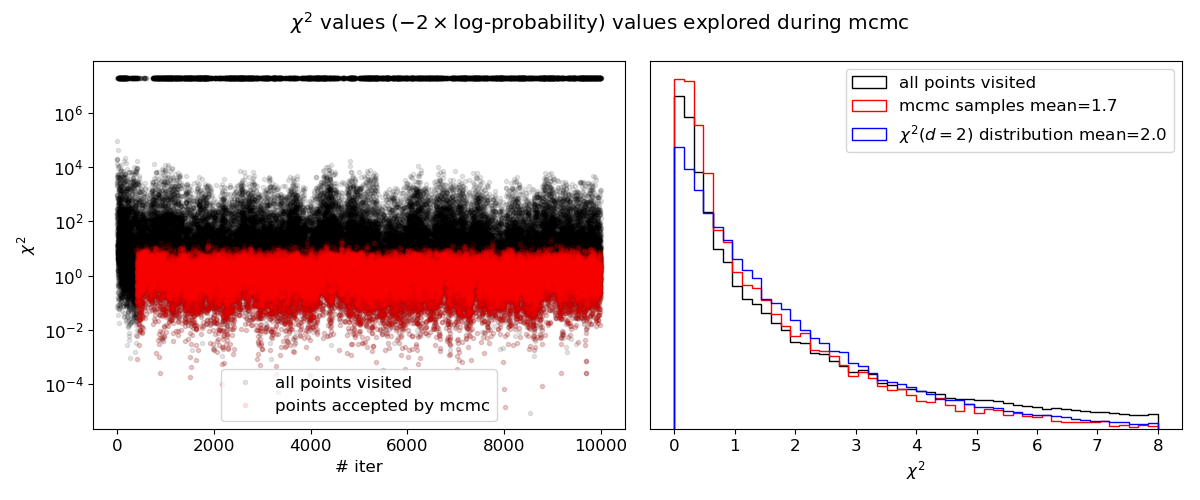
\includegraphics[width=\linewidth]{example_mcmc_log_probability_values_explore.png}
  \caption{The evolution of $\chi^2 = -2\log p$ during the run, and the histogram of accepted
           values (red) against a $\chi^2$ distribution with two degrees of freedom (blue). The
           numerically computed means are given in the legend; the analytic mean of the $\chi^2$
           distribution is the dimension.}
\end{figure}

The final product of the analysis is a \href{https://github.com/dfm/corner.py}{\texttt{corner}}
plot of the posterior, and its stability along the chain:

\begin{figure}[H]
  \centering
  \includegraphics[width=0.66\linewidth]{example_mcmc_parameters_distribution.png}
  \caption{The posterior: one- and two-dimensional marginals.}
\end{figure}

\begin{figure}[H]
  \centering
  \includegraphics[width=0.66\linewidth]{example_mcmc_parameters_distribution_convergence.png}
  \caption{The posterior as it would have been had the chains been stopped at five points along
           the run, from purple (earliest) to red (the full chain).}
\end{figure}

\section{MCMC against grid Monte Carlo}
\label{sec:mcmc-vs-mc}

How much does MCMC actually save? The target is minus the five-dimensional Rosenbrock function of
\cref{eq:rosenbrock}, sampled with $\Nc = 50$ walkers for $\Lc = 5\cdot 10^4$ iterations, starting
close to the known minimum.

\begin{figure}[H]
  \centering
  \includegraphics[width=0.72\linewidth]{example_mcmc_5d_parameters_distribution_convergence.png}
  \caption{The 5D posterior at five stopping points along the chains, without burn-in.}
\end{figure}

\begin{figure}[H]
  \centering
  \includegraphics[width=0.85\linewidth]{example_mcmc_5d_convergence_diagnostics.png}
  \caption{Convergence diagnostics of the 5D run, as in \cref{sec:mcmc-convergence}.}
\end{figure}

The same posterior is then computed by brute force, evaluating the density on a regular grid:

\begin{figure}[H]
  \centering
  \includegraphics[width=0.8\linewidth]{example_mcmc_and_mc_5d_parameters_distribution.png}
  \caption{The 5D posterior from MCMC (black) and from grid Monte Carlo (blue), and from a
           coarser grid with about as many samples as the MCMC (red). The legend gives the total
           number of samples and the computation time of each.}
\end{figure}

\begin{keypoint}[What the comparison shows]
The fine grid needs about $40\times$ more evaluations than MCMC for the same distribution, although
its total time was only about $2.5\times$ longer here, because MCMC carries more algorithmic
overhead per sample. Given the \emph{same} number of samples, the coarse grid is far from converged.
The gap widens rapidly with dimension --- and when each evaluation is an expensive simulation, it is
the number of evaluations, not the overhead, that counts.
\end{keypoint}
